\documentclass{standalone}
\usepackage{tikz}
\usetikzlibrary{patterns, positioning}
\usepackage[sfdefault]{ClearSans} %% option 'sfdefault' activates Clear Sans as the default text font
\usepackage[T1]{fontenc}

\begin{document}
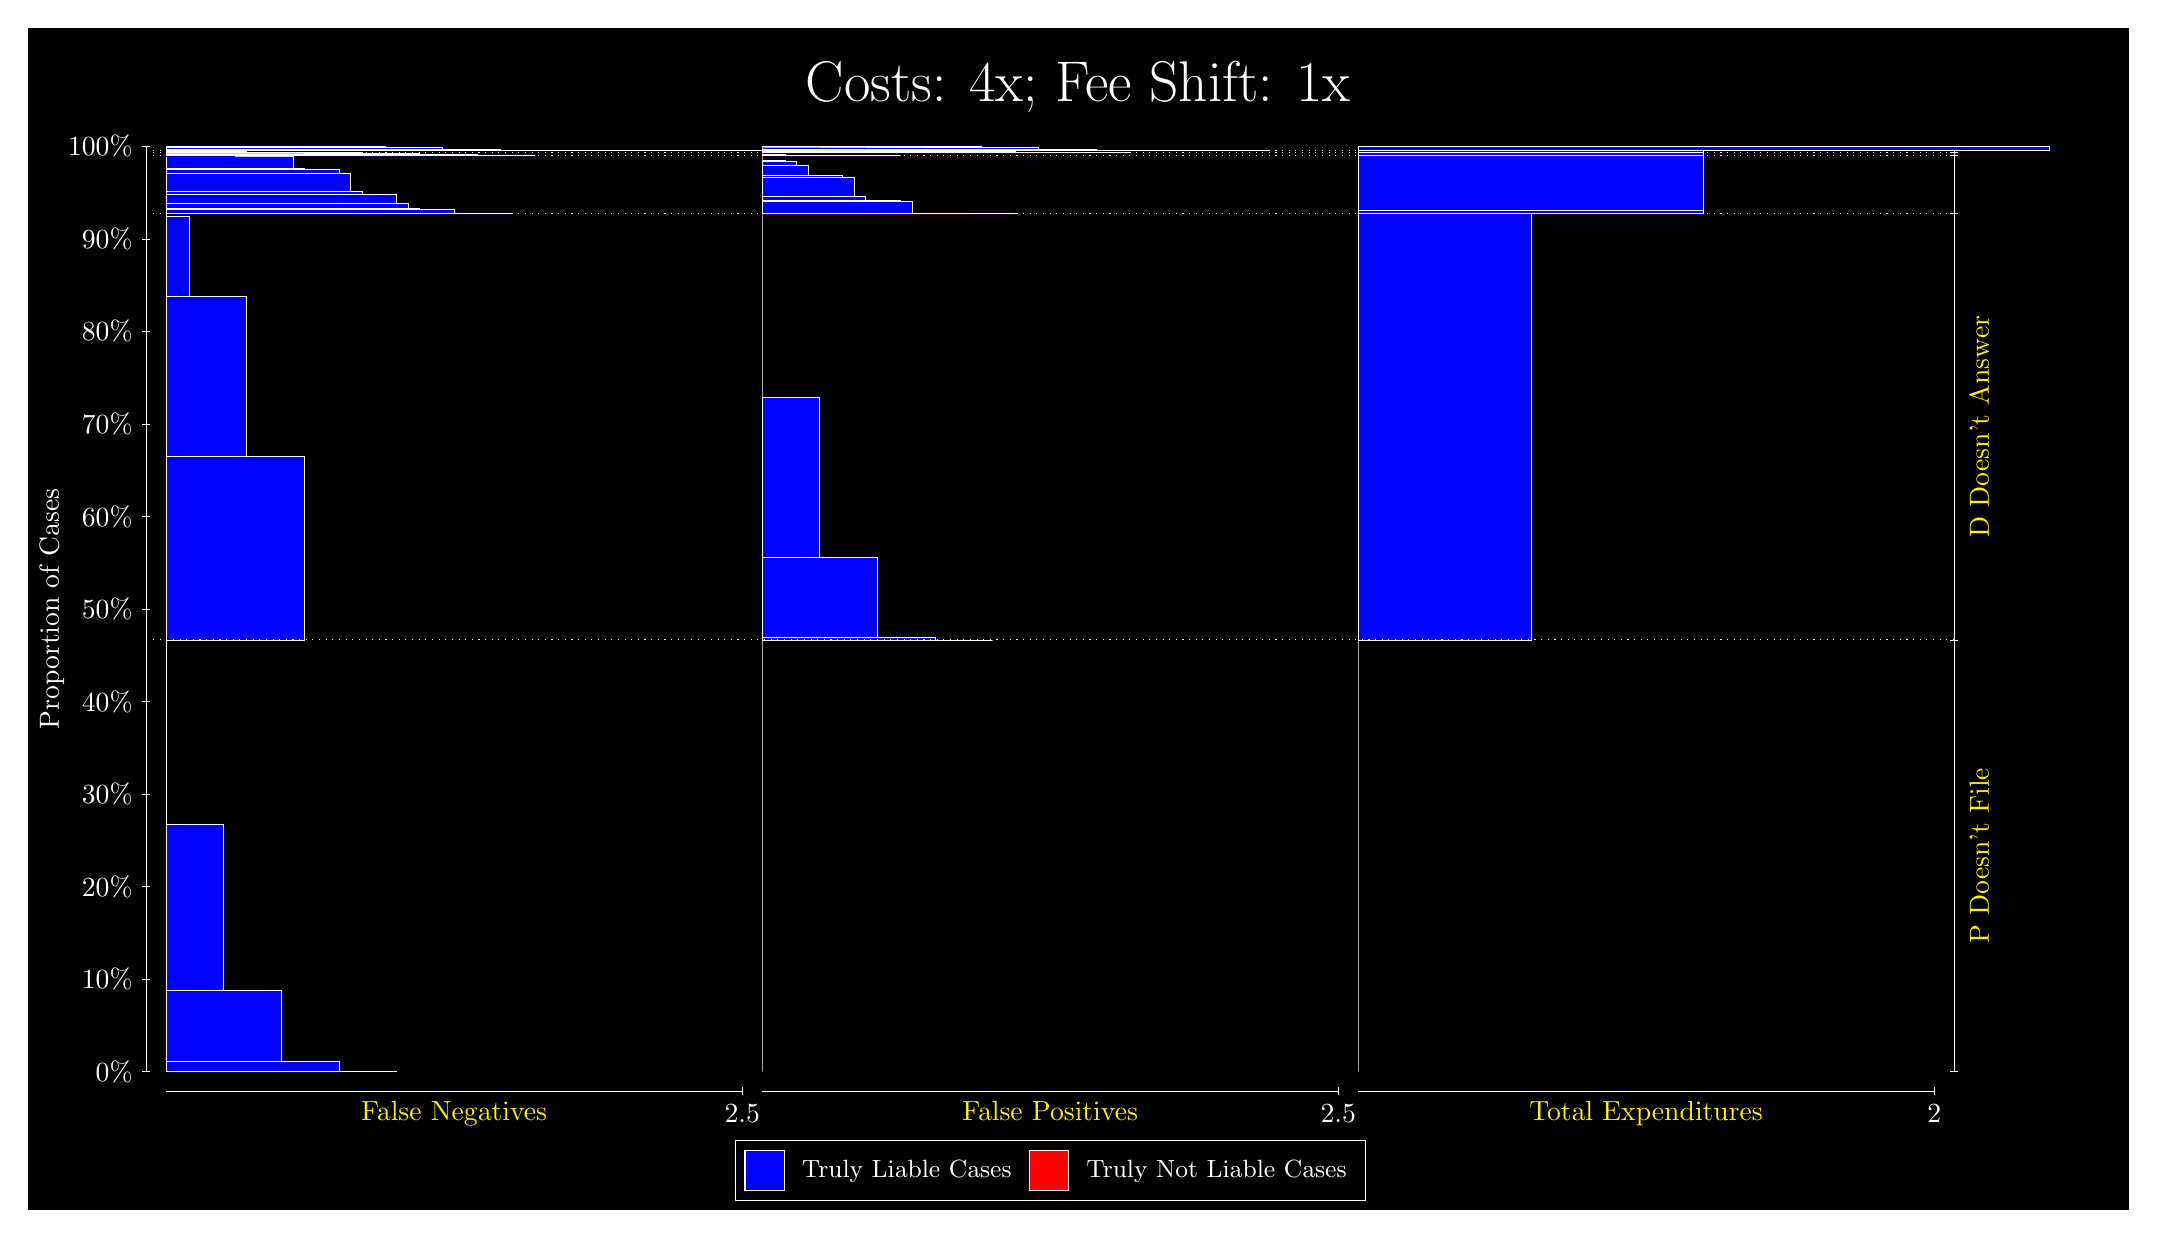
\begin{tikzpicture}
\draw[fill=black] (0,0) rectangle (26.667,15);
\draw[text=white] (0,13.5) rectangle (26.667,15) node[midway] {\huge Costs: 4x; Fee Shift: 1x};
\draw[white, very thin] (1.5,1.75) -- (1.5,13.5);
\node[rotate=90, text=white, anchor=center] at (0.3, 7.625) {Proportion of Cases};
\draw[white, very thin] (1.45,1.75) -- (1.55,1.75);
\node[text=white, anchor=east] at (1.45, 1.75) {0\%};
\draw[white, very thin] (1.45,2.925) -- (1.55,2.925);
\node[text=white, anchor=east] at (1.45, 2.925) {10\%};
\draw[white, very thin] (1.45,4.1) -- (1.55,4.1);
\node[text=white, anchor=east] at (1.45, 4.1) {20\%};
\draw[white, very thin] (1.45,5.275) -- (1.55,5.275);
\node[text=white, anchor=east] at (1.45, 5.275) {30\%};
\draw[white, very thin] (1.45,6.45) -- (1.55,6.45);
\node[text=white, anchor=east] at (1.45, 6.45) {40\%};
\draw[white, very thin] (1.45,7.625) -- (1.55,7.625);
\node[text=white, anchor=east] at (1.45, 7.625) {50\%};
\draw[white, very thin] (1.45,8.8) -- (1.55,8.8);
\node[text=white, anchor=east] at (1.45, 8.8) {60\%};
\draw[white, very thin] (1.45,9.975) -- (1.55,9.975);
\node[text=white, anchor=east] at (1.45, 9.975) {70\%};
\draw[white, very thin] (1.45,11.15) -- (1.55,11.15);
\node[text=white, anchor=east] at (1.45, 11.15) {80\%};
\draw[white, very thin] (1.45,12.325) -- (1.55,12.325);
\node[text=white, anchor=east] at (1.45, 12.325) {90\%};
\draw[white, very thin] (1.45,13.5) -- (1.55,13.5);
\node[text=white, anchor=east] at (1.45, 13.5) {100\%};

\draw[white, very thin] (24.457,1.75) -- (24.457,13.5);
\draw[white, very thin] (24.407,1.75) -- (24.507,1.75);
\node[anchor=west] at (24.407, 1.75) {};
\draw[white, very thin] (24.407,7.233) -- (24.507,7.233);
\node[anchor=west] at (24.407, 7.233) {};
\draw[white, very thin] (24.407,12.645) -- (24.507,12.645);
\node[anchor=west] at (24.407, 12.645) {};
\draw[white, very thin] (24.407,13.382) -- (24.507,13.382);
\node[anchor=west] at (24.407, 13.382) {};
\draw[white, very thin] (24.407,13.42) -- (24.507,13.42);
\node[anchor=west] at (24.407, 13.42) {};
\draw[white, very thin] (24.407,13.449) -- (24.507,13.449);
\node[anchor=west] at (24.407, 13.449) {};
\draw[white, very thin] (24.407,13.5) -- (24.507,13.5);
\node[anchor=west] at (24.407, 13.5) {};

\draw[white, very thin, fill=blue] (1.75,1.75) rectangle (4.6775,1.7513);
\draw[white, very thin, fill=blue] (1.75,1.7513) rectangle (3.9457,1.8778);
\draw[white, very thin, fill=blue] (1.75,1.8778) rectangle (3.2138,2.7855);
\draw[white, very thin, fill=blue] (1.75,2.7855) rectangle (2.4819,4.8855);
\draw[white, very thin, fill=red] (1.75,4.8855) rectangle (1.75,4.8855);
\draw[white, very thin, fill=blue] (1.75,4.8855) rectangle (1.75,7.233);
\draw[white, very thin, fill=blue] (1.75,7.233) rectangle (3.5065,9.5633);
\draw[white, very thin, fill=blue] (1.75,9.5633) rectangle (2.7746,11.597);
\draw[white, very thin, fill=blue] (1.75,11.597) rectangle (2.0428,12.61);
\draw[white, very thin, fill=red] (1.75,12.61) rectangle (1.75,12.61);
\draw[white, very thin, fill=blue] (1.75,12.61) rectangle (1.75,12.645);
\draw[white, very thin, fill=blue] (1.75,12.645) rectangle (6.1413,12.645);
\draw[white, very thin, fill=blue] (1.75,12.645) rectangle (5.5558,12.647);
\draw[white, very thin, fill=blue] (1.75,12.647) rectangle (5.4094,12.7);
\draw[white, very thin, fill=blue] (1.75,12.7) rectangle (4.9703,12.715);
\draw[white, very thin, fill=blue] (1.75,12.715) rectangle (4.8239,12.771);
\draw[white, very thin, fill=blue] (1.75,12.771) rectangle (4.6775,12.897);
\draw[white, very thin, fill=blue] (1.75,12.897) rectangle (4.2384,12.925);
\draw[white, very thin, fill=blue] (1.75,12.925) rectangle (4.092,13.162);
\draw[white, very thin, fill=blue] (1.75,13.162) rectangle (3.9457,13.214);
\draw[white, very thin, fill=blue] (1.75,13.214) rectangle (3.5065,13.219);
\draw[white, very thin, fill=blue] (1.75,13.219) rectangle (3.3602,13.379);
\draw[white, very thin, fill=blue] (1.75,13.379) rectangle (3.2138,13.38);
\draw[white, very thin, fill=blue] (1.75,13.38) rectangle (2.7746,13.38);
\draw[white, very thin, fill=blue] (1.75,13.38) rectangle (2.6283,13.382);
\draw[white, very thin, fill=blue] (1.75,13.382) rectangle (2.0428,13.382);
\draw[white, very thin, fill=red] (1.75,13.382) rectangle (1.75,13.382);
\draw[white, very thin, fill=blue] (1.75,13.382) rectangle (6.4341,13.382);
\draw[white, very thin, fill=blue] (1.75,13.382) rectangle (5.7022,13.397);
\draw[white, very thin, fill=blue] (1.75,13.397) rectangle (4.9703,13.418);
\draw[white, very thin, fill=blue] (1.75,13.418) rectangle (4.2384,13.42);
\draw[white, very thin, fill=blue] (1.75,13.42) rectangle (3.5065,13.42);
\draw[white, very thin, fill=red] (1.75,13.42) rectangle (1.75,13.42);
\draw[white, very thin, fill=blue] (1.75,13.42) rectangle (3.5065,13.42);
\draw[white, very thin, fill=blue] (1.75,13.42) rectangle (2.7746,13.437);
\draw[white, very thin, fill=blue] (1.75,13.437) rectangle (2.0428,13.449);
\draw[white, very thin, fill=red] (1.75,13.449) rectangle (1.75,13.449);
\draw[white, very thin, fill=blue] (1.75,13.449) rectangle (1.75,13.449);
\draw[white, very thin, fill=blue] (1.75,13.449) rectangle (11.704,13.449);
\draw[white, very thin, fill=blue] (1.75,13.449) rectangle (10.972,13.449);
\draw[white, very thin, fill=blue] (1.75,13.449) rectangle (10.24,13.45);
\draw[white, very thin, fill=blue] (1.75,13.45) rectangle (9.508,13.453);
\draw[white, very thin, fill=blue] (1.75,13.453) rectangle (8.7761,13.453);
\draw[white, very thin, fill=blue] (1.75,13.453) rectangle (8.0442,13.453);
\draw[white, very thin, fill=blue] (1.75,13.453) rectangle (7.4587,13.453);
\draw[white, very thin, fill=blue] (1.75,13.453) rectangle (6.7268,13.453);
\draw[white, very thin, fill=blue] (1.75,13.453) rectangle (5.9949,13.462);
\draw[white, very thin, fill=blue] (1.75,13.462) rectangle (5.2631,13.488);
\draw[white, very thin, fill=blue] (1.75,13.488) rectangle (4.5312,13.499);
\draw[white, very thin, fill=blue] (1.75,13.499) rectangle (3.7993,13.5);
\draw[white, very thin, fill=blue] (1.75,13.5) rectangle (3.0674,13.5);
\draw[white, very thin, fill=blue] (1.75,13.5) rectangle (2.3355,13.5);
\draw[white, very thin, fill=red] (1.75,13.5) rectangle (1.75,13.5);
\draw[white, very thin, fill=red] (9.3189,1.75) rectangle (9.3189,1.75);
\draw[white, very thin, fill=blue] (9.3189,1.75) rectangle (9.3189,7.233);
\draw[white, very thin, fill=red] (9.3189,7.233) rectangle (12.246,7.233);
\draw[white, very thin, fill=blue] (9.3189,7.233) rectangle (12.246,7.233);
\draw[white, very thin, fill=blue] (9.3189,7.233) rectangle (11.515,7.2676);
\draw[white, very thin, fill=blue] (9.3189,7.2676) rectangle (10.783,8.2806);
\draw[white, very thin, fill=blue] (9.3189,8.2806) rectangle (10.051,10.314);
\draw[white, very thin, fill=blue] (9.3189,10.314) rectangle (9.3189,12.645);
\draw[white, very thin, fill=red] (9.3189,12.645) rectangle (12.539,12.645);
\draw[white, very thin, fill=blue] (9.3189,12.645) rectangle (12.539,12.645);
\draw[white, very thin, fill=red] (9.3189,12.645) rectangle (11.954,12.645);
\draw[white, very thin, fill=blue] (9.3189,12.645) rectangle (11.954,12.647);
\draw[white, very thin, fill=blue] (9.3189,12.647) rectangle (11.807,12.647);
\draw[white, very thin, fill=red] (9.3189,12.647) rectangle (11.368,12.647);
\draw[white, very thin, fill=blue] (9.3189,12.647) rectangle (11.368,12.647);
\draw[white, very thin, fill=blue] (9.3189,12.647) rectangle (11.222,12.807);
\draw[white, very thin, fill=blue] (9.3189,12.807) rectangle (11.075,12.812);
\draw[white, very thin, fill=blue] (9.3189,12.812) rectangle (10.636,12.864);
\draw[white, very thin, fill=blue] (9.3189,12.864) rectangle (10.49,13.101);
\draw[white, very thin, fill=blue] (9.3189,13.101) rectangle (10.344,13.129);
\draw[white, very thin, fill=blue] (9.3189,13.129) rectangle (9.9044,13.255);
\draw[white, very thin, fill=blue] (9.3189,13.255) rectangle (9.758,13.311);
\draw[white, very thin, fill=blue] (9.3189,13.311) rectangle (9.6116,13.326);
\draw[white, very thin, fill=blue] (9.3189,13.326) rectangle (9.3189,13.382);
\draw[white, very thin, fill=red] (9.3189,13.382) rectangle (11.075,13.382);
\draw[white, very thin, fill=blue] (9.3189,13.382) rectangle (11.075,13.382);
\draw[white, very thin, fill=blue] (9.3189,13.382) rectangle (10.344,13.384);
\draw[white, very thin, fill=blue] (9.3189,13.384) rectangle (9.6116,13.405);
\draw[white, very thin, fill=blue] (9.3189,13.405) rectangle (9.3189,13.42);
\draw[white, very thin, fill=red] (9.3189,13.42) rectangle (14.003,13.42);
\draw[white, very thin, fill=blue] (9.3189,13.42) rectangle (14.003,13.42);
\draw[white, very thin, fill=blue] (9.3189,13.42) rectangle (13.271,13.42);
\draw[white, very thin, fill=blue] (9.3189,13.42) rectangle (12.539,13.432);
\draw[white, very thin, fill=blue] (9.3189,13.432) rectangle (11.807,13.449);
\draw[white, very thin, fill=blue] (9.3189,13.449) rectangle (11.075,13.449);
\draw[white, very thin, fill=red] (9.3189,13.449) rectangle (15.759,13.449);
\draw[white, very thin, fill=blue] (9.3189,13.449) rectangle (15.759,13.449);
\draw[white, very thin, fill=blue] (9.3189,13.449) rectangle (15.028,13.449);
\draw[white, very thin, fill=red] (9.3189,13.449) rectangle (15.028,13.449);
\draw[white, very thin, fill=blue] (9.3189,13.449) rectangle (15.028,13.449);
\draw[white, very thin, fill=blue] (9.3189,13.449) rectangle (14.296,13.45);
\draw[white, very thin, fill=red] (9.3189,13.45) rectangle (14.296,13.45);
\draw[white, very thin, fill=blue] (9.3189,13.45) rectangle (14.296,13.45);
\draw[white, very thin, fill=blue] (9.3189,13.45) rectangle (13.564,13.455);
\draw[white, very thin, fill=red] (9.3189,13.455) rectangle (13.564,13.455);
\draw[white, very thin, fill=blue] (9.3189,13.455) rectangle (13.564,13.461);
\draw[white, very thin, fill=blue] (9.3189,13.461) rectangle (12.832,13.462);
\draw[white, very thin, fill=blue] (9.3189,13.462) rectangle (12.832,13.487);
\draw[white, very thin, fill=blue] (9.3189,13.487) rectangle (12.1,13.496);
\draw[white, very thin, fill=blue] (9.3189,13.496) rectangle (11.368,13.496);
\draw[white, very thin, fill=blue] (9.3189,13.496) rectangle (10.636,13.496);
\draw[white, very thin, fill=red] (9.3189,13.496) rectangle (10.051,13.496);
\draw[white, very thin, fill=blue] (9.3189,13.496) rectangle (10.051,13.496);
\draw[white, very thin, fill=red] (9.3189,13.496) rectangle (9.3189,13.496);
\draw[white, very thin, fill=blue] (9.3189,13.496) rectangle (9.3189,13.5);
\draw[white, very thin, fill=red] (16.888,1.75) rectangle (16.888,1.75);
\draw[white, very thin, fill=blue] (16.888,1.75) rectangle (16.888,7.233);
\draw[white, very thin, fill=red] (16.888,7.233) rectangle (19.083,7.233);
\draw[white, very thin, fill=blue] (16.888,7.233) rectangle (19.083,12.645);
\draw[white, very thin, fill=red] (16.888,12.645) rectangle (21.279,12.645);
\draw[white, very thin, fill=blue] (16.888,12.645) rectangle (21.279,12.692);
\draw[white, very thin, fill=red] (16.888,12.692) rectangle (21.279,12.692);
\draw[white, very thin, fill=blue] (16.888,12.692) rectangle (21.279,13.382);
\draw[white, very thin, fill=red] (16.888,13.382) rectangle (21.279,13.382);
\draw[white, very thin, fill=blue] (16.888,13.382) rectangle (21.279,13.42);
\draw[white, very thin, fill=red] (16.888,13.42) rectangle (21.279,13.42);
\draw[white, very thin, fill=blue] (16.888,13.42) rectangle (21.279,13.449);
\draw[white, very thin, fill=red] (16.888,13.449) rectangle (25.67,13.449);
\draw[white, very thin, fill=blue] (16.888,13.449) rectangle (25.67,13.455);
\draw[white, very thin, fill=red] (16.888,13.455) rectangle (25.67,13.455);
\draw[white, very thin, fill=blue] (16.888,13.455) rectangle (25.67,13.5);
\draw[white, dotted] (1.5,7.233) -- (24.457,7.233);
\draw[white, dotted] (1.5,12.645) -- (24.457,12.645);
\draw[white, dotted] (1.5,13.382) -- (24.457,13.382);
\draw[white, dotted] (1.5,13.42) -- (24.457,13.42);
\draw[white, dotted] (1.5,13.449) -- (24.457,13.449);
\draw[white, very thin] (1.75,1.5) -- (9.0689,1.5);
\node[text=yellow, anchor=north] at (5.4094, 1.5) {False Negatives};
\draw[white, very thin] (9.0689,1.45) -- (9.0689,1.55);
\node[text=white, anchor=north] at (9.0689, 1.45) {2.5};

\draw[white, very thin] (9.3189,1.5) -- (16.638,1.5);
\node[text=yellow, anchor=north] at (12.978, 1.5) {False Positives};
\draw[white, very thin] (16.638,1.45) -- (16.638,1.55);
\node[text=white, anchor=north] at (16.638, 1.45) {2.5};

\draw[white, very thin] (16.888,1.5) -- (24.207,1.5);
\node[text=yellow, anchor=north] at (20.547, 1.5) {Total Expenditures};
\draw[white, very thin] (24.207,1.45) -- (24.207,1.55);
\node[text=white, anchor=north] at (24.207, 1.45) {2};

\node[text=yellow, centered, rotate=90] at (24.777, 4.4915) {P Doesn't File};
\node[text=yellow, centered, rotate=90] at (24.777, 9.9388) {D Doesn't Answer};





\draw (12.978300999999998,1.5) node[draw=none] (baseCoordinate) {};
\begin{scope}[align=center]
        \matrix[scale=0.5, draw=white, below=0.5cm of baseCoordinate, nodes={draw}, column sep=0.1cm]{
            \node[rectangle, draw, minimum width=0.5cm, minimum height=0.5cm, fill=blue] {}; &
            \node[draw=none, font=\small, text=white] (B) {Truly Liable Cases}; &
            \node[rectangle, draw, minimum width=0.5cm, minimum height=0.5cm, fill=red] {}; &
            \node[draw=none, font=\small, text=white] (B) {Truly Not Liable Cases}; \\
            };
\end{scope}

\end{tikzpicture}
\end{document}